\subsection{WIMP Interface}
Contemporary GUIs are sometimes called ''WIMP” (Windows, Icons, Menus, Pointers) interfaces. Multiple windows can pose management difficulties. There are two types of window managers: The operating system software and the user who must minimize, maximize, resize, access, and organize windows. Studies have shown that the advantages offered by windowing systems can be negated by excess window manipulation requirements.
Window Managers are responsible for a common look-and-feel. This look-and-feel is either embedded into the operating system (Windows, MacOS) or kept separate (Unix). Most windowing systems use standardized windows that look similar and behave consistently.\\
\begin{figure}[h!]
	\centering
	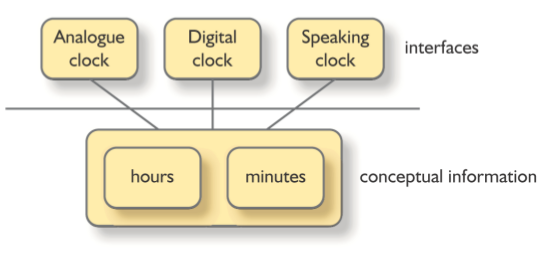
\includegraphics[width=.4\textwidth]{img/ch07_con.png}
	\caption{The same conceptual information can be presented via different physical interfaces.}
	\label{con}
\end{figure}
How is a information presented to the user in term of Form, Structure, and Content/Description? The decision determines which information/action is easier to access and which is more difficult to access. There are various was to arrange windows: Tiled windows afford drag-and-drop methods. Overlapping windows use screen real estate efficiently, but they can become overwhelming. Cascading windows use screen real estate efficiently and can be used to create visual organization. Maximized windows are visually less complex, but they require easy navigation methods to get from window to window. Tabs increase the size of the dialogue by stacking layers on top of each other. Stacked tabs move around to accommodate the different levels and they destroy location consistency.
\subsection{Text and Reading}
The Reading Process can be monitored in term of saccades (quick, jerky eye movements, about 8-10 letters) and fixations (intermittent pauses on areas of interest). Visual and cognitive processing occurs during fixation but not during saccades. If text is difficult to comprehend, if it includes long or unfamiliar words, fixations increase in duration. Reading is a 2-step process:\\
1) distinguish letter or word shapes (only experienced readers recognize word shapes)\\
2) Associate meaning\\\\
Some known human issues concerning text/reading:
\begin{itemize}
\item Readers do not have much trouble reading texts where the letters of the individual words are jumbled, as long as the first and last letter of each word remain in place.
\item Single letters are simpler identifiable if they are in uppercase
\item We read extended text passages more quickly in lowercase than uppercase
\item Lowercase presentation is more common. Lowercase words have more distinctive shapes.
\item Reading a novel is a continuous process. For many other texts we use scanning
\item Reading from screens or paper is different: We often rely on our spatial memory when we search for information (Web-Problem!). On paper, the ability to annotate aids comprehension.
\end{itemize}
In interaction design, text is either used in two ways:
\begin{itemize}
\item Commentary -- Text that informs: The most common form is help text.
\begin{itemize}
\item Contextual help provides immediate assistance to users without requiring them to leave the context in which they are working, such as pop-up menus.
\item Procedural help provides the steps necessary for carrying out a task.
\item Reference help serves as an online reference book.
\item Conceptual help provides background information, feature overviews, or processes
\end{itemize} 
\item Instrumental -- Text that does work: Controls (Buttons, Checkboxes, Radio Buttons, Icons, Hyperlinks) have labels which form one entity with their respective function. E.g. Hypertext links must give unambiguous indications of the target destination.
\end{itemize}
Other Design Issues are Legibility (Age, context determine size, contrast etc.), Readability (comprehension is affected by Line length, Line spacing, Formatting, Margin width, Scrolling and also by grammatical issues, such as semantics and syntax) and \textbf{Physical Factors}:
\begin{itemize}
\item Font size: 9-12pts are equally readable (Dix et al.); several factors affect font size according to Horton:
\begin{itemize}
\item Reading Distance: Greater distances require larger text.
\item Screen Resolution: Smaller text requires greater resolution to keep the characters clear and legible.
\item Text/Background Contrast: Negative contrast is optimal (black type on a white background).
\item Visual Acuity of User: Age, Abilities etc.
\item Type of Reading: Text can be scanned, read word by word, or read character by character
\end{itemize}
\item Line length: affects reading performance but not comprehension. Lines of greater length are read more quickly. People prefer medium line lengths.
\item Margin width: Shorter lines with large margins increase reading performance (Maximal use of white space)
\item Vertical line spacing: The spacing between lines of text (single spacing, double spacing, etc.) is called leading. Double spacing has been shown to improve reading speed. However, it might necessitate a smaller font size to increase the amount of visible information per screen.
\item Alignment: For optimal reading of lengthy texts, right and center alignments should be avoided. Text should also be considered a graphical component of a page.
\item Contrast: Contrast sensitivity decreases significantly with age. Because black and white have the highest contrast the addition of any color will reduce the contrast. Luminance contrast is more significant than color contrast.
\item Scrolling versus paging: Which is better depends on application.
\end{itemize}
\textbf{Fonts}: Serif fonts guide the reader. Thus they are suitable for long text lines e.g. in books. Non-serif fonts are less complex to recognize (less elements), thus they are more suitable for cases where fast recognition is important, e.g. presentation slides. Cursive text is similar to hand written text and requires high-resolution screens. One further distinguished between variable-width and fixed-width fonts. In the latter, each character takes up the same horizontal width ($\rightarrow$ more whitespace in between letters).
There are good (most of them expensive) and cheap fonts (E.g. Arial is a cheap version of Helvetica). Font creation and readability of fonts is a science of its own.

\subsection{Information}
The Information Architecture structures the presented information, thus influencing the conceptualization of the user. Ontologies define the concept of information. How we group things together/ classify them is the concern of taxonomy. Information should be presented consistently (i.e. using one taxonomy), but we know that in practice several taxonomies can coexist.\\
Two general ways for structuring:
\begin{itemize}
\item Coarse-grained: The general information structure provides many objects to be selected. This reduces the number of steps until you reach the object in question. Example: One HTML document containing several sections
\item Fine-grained: There are fine-grained objects, that are reached through a sophisticated, often multi-step process (e.g. through several menus). Example: One HTML document per section
\end{itemize}
How to build information structure: 
\begin{itemize}
\item Volatility: Select an ontology that stays stable, e.g. so you do not have to change your menu logic
\item Size: Decide if moving in an object is more suitable than moving between objects, e.g. scrolling vs. forward-next clicking (experts prefer scrolling)
\item Conceptual / physical mapping: Information must be suitable to all input/output devices ($\rightarrow$ 20 Menu buttons on mobile phone?)
\item Topology: Most important also for Web, determines how easy it is to move through information space (e.g. a Web-Site). Distance is the number of clicks needed for navigation. Direction plays a role for navigation, e.g. an Audio Interface has often only forward navigation
\end{itemize}
In information design it is also important to use one consistent classification scheme, e.g. Alphabetical, Chronological, Geographical (e.g. travel agent: ``Germany''), Topic (e.g. Cars, Repairs), Task-based (``buy a car'',''repair a car''), Audience (Car Buyers), Semantic (Functions, Objects etc. separated)

\subsection{Interaction}
There are many interaction styles: 
\begin{itemize}
\item Command Line: You need to recall information, not recognize it. But it is also simpler to remember words than graphical interface elements. We need a very good concept of use. Steep learning curve, thus better for expert users. Repetition of tasks is simpler. Complexity can be handled easy through concatenation etc. In general faster for complex tasks. But higher error rate, higher cognitive load.
\item Menu-Based Interface: Function can be recognized, position/structure recalled. Menus may be graphical or textual. Much better for seldom used functions, self explanatory. Range of possible options shown $\rightarrow$ constraints. Allows a user to build a concept of the system. Menu Types include Single, Sequential, Hierarchical and Network / Meshed menus.
\item Form Fill-In: Special for gathering strings of information. Linear, not related to navigation. It is important that the users know how long the form will be, and where he is. Errors are problematic, annoy the user. Unambiguous labeling is important to preserve data integrity. Input formats may vary (e.g. how to enter a date?)
\item Wizards/Question and Answer: Form with flow for beginners. Often represents ``most used'' design flow. Present only very restricted information at one time. Very restricted in control flow, thus inappropriate for any input where a great variety of control flows exist. BUT: Today omnipresent in many applications, because most users are beginners at some point (e.g. installation time) for programs. Or always, because of infrequent use.
\item Direct Manipulation/Metaphors (Ben Sheiderman, 1982): Continuous representations of objects and actions of interest with meaningful visual metaphors. Simple physical actions to perform manipulations. Rapid, incremental, reversible actions whose effects on objects are visible immediately. Metaphors are most critical: They allow a user to understand a concept without or with reduced learning, often using real-world associations. However, they are not always consistent and simplifying. Also, different people have various concepts for the same objects. Touch interaction is also a form of direct manipulation.
\item Web Navigation
\item Three-Dimensional Environments
\item Zoomable Interface
\item Natural Language
\end{itemize}
\textbf{Object-Action model}: The user first selects an object and then selects the action to be performed on the selected object (e.g. MAC user interface).\\\\
\textbf{Action-Object model}: The user first selects an action to be performed and then selects the objects on which this action will be performed (e.g. typical Windows usage).